%% Modelo UNISINOS para Trabalhos de Conclusão de Curso (TCCs) baseado no abtex2-modelo-trabalho-academico.tex, v-1.9.5 laurocesar Copyright 2012-2015 by abnTeX2 group at http://www.abntex.net.br/ 
% ----------------------------------------------
% abnTeX2: Modelo de Trabalho Academico (tese de doutorado, dissertacao de mestrado e trabalhos monograficos em geral) em conformidade com ABNT NBR 14724:2011: Informacao e documentacao - Trabalhos academicos - Apresentacao
% ----------------------------------------------
% ==============================================
% ||||||||||||||||||||||||||||||||||||||||||||||
% ----------------------------------------------
\documentclass[
	% -- opções da classe memoir --
	12pt,				% tamanho da fonte
	openright,			% capítulos começam em pág ímpar (insere página vazia caso preciso)
	oneside,			% para impressão em verso e anverso. twoside Oposto a oneside
	a4paper,			% tamanho do papel. 
	% -- opções da classe abntex2 --
	chapter=TITLE,		% títulos de capítulos convertidos em letras maiúsculas
	%section=TITLE,		% títulos de seções convertidos em letras maiúsculas
	%subsection=TITLE,	% títulos de subseções convertidos em letras maiúsculas
	%subsubsection=TITLE,% títulos de subsubseções convertidos em letras maiúsculas
	% -- opções do pacote babel --
	english,			% idioma adicional para hifenização
%	french,				% idioma adicional para hifenização
%	spanish,			% idioma adicional para hifenização
	brazil				% o último idioma é o principal do documento
	]{abntex2} 
% ----------------------------------------------
% Pacotes de fontes... 
% ----------------------------------------------
\renewcommand{\ABNTEXchapterfont}{\fontfamily{ptm}\fontseries{sbc}\selectfont}
% \usepackage{lmodern}	% Usa a fonte Latin Modern
% \usepackage{fourier}	% Adobe utopia
% \usepackage{times}	% Usa a fonte Times, mas não muito boa
% \usepackage{palatino}	% Usa a fonte Palatino
% \usepackage{mathpazo}	% Usa a fonte Adobe Palatino

% \usepackage[scaled=.92]{helvet} % Usa a fonte Helvetica
% % Descomente a linha abaixo junto se for utilizar a fonte helvet
% \renewcommand{\familydefault}{\sfdefault}
\usepackage{mathptmx}
%\usepackage{tgtermes}
% Para entradas de capítulo com Times Bold usando um dos 2 pacotes acima
% \renewcommand{\ABNTEXchapterfont}{\rmfamily\bfseries}
% ----------------------------------------------
% Configuração das fontes
% ----------------------------------------------
% Algumas configurações de fontes para capitulos e seções tanto no texto quanto no sumário
\renewcommand{\ABNTEXchapterfont}{\bfseries}
\renewcommand{\ABNTEXchapterfontsize}{\Large}
\renewcommand{\ABNTEXpartfont}{\ABNTEXchapterfont}
\renewcommand{\ABNTEXpartfontsize}{\ABNTEXchapterfontsize}
\renewcommand{\cftpartfont}{\normalfont\bfseries}
\renewcommand{\ABNTEXsectionfont}{\bfseries}
\renewcommand{\ABNTEXsectionfontsize}{\large}
\renewcommand{\ABNTEXsubsectionfont}{\normalfont}
\renewcommand{\ABNTEXsubsectionfontsize}{\normalsize}
\renewcommand{\cftsubsectionfont}{\normalfont}
\renewcommand{\ABNTEXsubsubsectionfont}{\slshape}
\renewcommand{\cftsubsubsectionfont}{\normalfont\slshape}
\renewcommand{\ABNTEXsubsubsubsectionfont}{\bfseries}
% Para configurar mais níveis configure conforme utilizado acima e comente as duas linhas abaixo
\settocdepth{subsubsection} % configura sumário para apresentar subseções até o quarto nível
\setsecnumdepth{subsubsection} % configura para numerar subseções até o quarto nível. Subseções de quinto nível não conterão numeração.
\addto\captionsbrazil{\renewcommand{\listfigurename}{Lista de figuras}} % Altera nome da lista de ilustrações para lista de figuras
% \addto{\captionsbrazil}{\renewcommand{\bibname}{Referências Bibliográficas}}
% ----------------------------------------------
% Equações com numeração sequencial
% ----------------------------------------------
\usepackage{chngcntr}
\counterwithout{equation}{chapter}
% ----------------------------------------------
% Pacotes básicos 
% ----------------------------------------------
\usepackage[T1]{fontenc}	% Selecao de codigos de fonte.
\usepackage[utf8]{inputenc}	% Codificacao do documento (conversão automática dos acentos)
\usepackage{lastpage}		% Usado pela Ficha catalográfica
\usepackage{indentfirst} 	% Indenta o primeiro parágrafo de cada seção.
\usepackage{color, colortbl}% Controle das cores
\usepackage{float}
\usepackage{graphicx}		% Inclusão de gráficos
\usepackage{microtype} 		% para melhorias de justificação
\usepackage{array}
%\usepackage{gensymb}       % Símbolos
\usepackage{amsmath} 	%--------------------------%
\usepackage{hyperref} 	%--------------------------%
\usepackage{bibentry} 	% para inserir refs. bib. no meio do texto
% ----------------------------------------------
% Pacotes adicionais
% ----------------------------------------------
\usepackage{lipsum}	% para geração de dummy text
\usepackage[colorinlistoftodos, english]{todonotes}
  % exemplos de uso: 
  %\todo[inline, color=red!80]{texto}
\usepackage{verbatim}
\usepackage{soulutf8}
  % exemplos de uso: 
  %\hl{highlight} ou \st{strikeout} ou \ul{underline}
\usepackage{tabularx}
\usepackage{multirow}
%\usepackage{subfig}
\usepackage{pdfpages}
\usepackage{pgfplots}
  \pgfplotsset{compat=1.12}
% Para desenho de circuitos
\usepackage{tikz}
\usepackage[american]{circuitikz}
\usepackage{siunitx}
\sisetup{locale = FR}

% ---
% Formatação de código-fonte
% ---
\usepackage{listings}

% Altera o nome padrão do rótulo usado no comando \autoref{}
\renewcommand{\lstlistingname}{Código}

% Altera o rótulo a ser usando no elemento pré-textual "Lista de código"
\renewcommand{\lstlistlistingname}{Lista de códigos}

% Configura a ``Lista de Códigos'' conforme as regras da ABNT (para abnTeX2)
\begingroup\makeatletter
\let\newcounter\@gobble\let\setcounter\@gobbletwo
  \globaldefs\@ne \let\c@loldepth\@ne
  \newlistof{listings}{lol}{\lstlistlistingname}
  \newlistentry{lstlisting}{lol}{0}
\endgroup

\renewcommand{\cftlstlistingaftersnum}{\hfill--\hfill}

\let\oldlstlistoflistings\lstlistoflistings
\renewcommand{\lstlistoflistings}{%
   \begingroup%
   \let\oldnumberline\numberline%
   \renewcommand{\numberline}{\lstlistingname\space\oldnumberline}%
   \oldlstlistoflistings%
   \endgroup}



\usepackage{color}
\definecolor{dkgreen}{rgb}{0,0.6,0}
\definecolor{gray}{rgb}{0.5,0.5,0.5}
\definecolor{mauve}{rgb}{0.58,0,0.82}
\lstset{frame=tb,
  language=C,
  aboveskip=3mm,
  belowskip=3mm,
  showstringspaces=false,
  columns=flexible,
  basicstyle={\small\ttfamily},
  numbers=left,
  numberstyle=\tiny\color{gray},
  keywordstyle=\color{blue},
  commentstyle=\color{dkgreen},
  stringstyle=\color{mauve},
  breaklines=true,
  breakatwhitespace=true,
  tabsize=3
}     
% ----------------------------------------------
% Pacotes de citações
% ----------------------------------------------
\usepackage[brazilian,hyperpageref]{backref}	 % Paginas com as citações na bibl
\usepackage[alf, abnt-etal-text=it]{abntex2cite} % Citações padrão ABNT
% ==============================================
% CONFIGURAÇÕES DE PACOTES
% ==============================================
% ----------------------------------------------
% Configurações do pacote backref
% Usado sem a opção hyperpageref de backref
% ----------------------------------------------
\renewcommand{\backrefpagesname}{Citado na(s) página(s):~}
% Texto padrão antes do número das páginas
\renewcommand{\backref}{}
% Define os textos da citação
\renewcommand*{\backrefalt}[4]{
	\ifcase #1 %
		Nenhuma citação no texto.%
	\or
		Citado na página #2.%
	\else
		Citado #1 vezes nas páginas #2.%
	\fi}%
% ||||||||||||||||||||||||||||||||||||||||||||||
% Informações de dados para CAPA e FOLHA DE ROSTO
% ||||||||||||||||||||||||||||||||||||||||||||||
\titulo{DETECÇÃO E DIAGNÓSTICO AUTOMÁTICO DE FALHAS EM MOTORES ELÉTRICOS DE INDUÇÃO VIA ANÁLISE DE ASSINATURAS NA CORRENTE ELÉTRICA E VIBRAÇÃO}
\autor{GUILHERME ANGELO PIAIA}
\local{São Leopoldo, RS}
\data{2021}
\orientador{Prof. Dr. Rodrigo Marques de Figueiredo} 
%Nome completo do professor com sua titulação (Esp. ou MS. ou Dr.)
%\coorientador{Prof. Dr. }
\instituicao{%
  UNIVERSIDADE DO VALE DO RIO DOS SINOS - UNISINOS
  \par
  UNIDADE ACADÊMICA DE PESQUISA E PÓS-GRADUAÇÃO
  \par
  PROGRAMA DE PÓS-GRADUAÇÃO EM ENGENHARIA ELÉTRICA
  \par
  NÍVEL MESTRADO PROFISSIONAL}

\tipotrabalho{Dissertação (Mestrado)}
% O preambulo deve conter o tipo do trabalho, o objetivo, o nome da instituição e a área de concentração 
% Verifique a nomenclatura utilizada: Graduado, Bacharel ou Licenciado junto à Coordenação do seu Curso.
\preambulo{Dissertação apresentada como requisito parcial para obtenção do título de Mestre em Engenharia Elétrica,
 pelo Programa de Pós-Graduação em Engenharia Elétrica da Universidade do Vale do Rio dos Sinos - UNISINOS.}
% ----------------------------------------------
% Configurações de aparência do PDF final
% ----------------------------------------------
% alterando o aspecto da cor azul
\definecolor{blue}{RGB}{41,5,195}
% alterando o aspecto da cor cinza
\definecolor{gray}{RGB}{50,50,50}
% informações do PDF
\makeatletter
\hypersetup{
    %pagebackref=true,
    pdftitle={\imprimirtitulo}, 
    pdfauthor={\imprimirautor},
    pdfsubject={\imprimirpreambulo},
	pdfcreator={LaTeX - abnTeX2 - Overleaf},
	pdfkeywords={abnt}{latex}{abntex2}{trabalho acadêmico}{unisinos}{engenharia de controle e automação}{tcc},
    colorlinks=true, % false: boxed links; true: colored links
    linkcolor=black, % color of internal links
    citecolor=black, % color of links to bibliography
    filecolor=blue,  % color of file links
    urlcolor=gray,
    bookmarksdepth=4
}
\makeatother
% ----------------------------------------------
% Espaçamentos entre linhas e parágrafos 
% ----------------------------------------------
% O tamanho do parágrafo é dado por:
\setlength{\parindent}{1.3cm}
% Controle do espaçamento entre um parágrafo e outro:
\setlength{\parskip}{0.2cm}  % tente também \onelineskip
% ----------------------------------------------
% compila o indice
% ----------------------------------------------
\makeindex

% ----------------------------------------------
% Pacotes extras
% ----------------------------------------------
%\newcommand*\cuk{\´{C}}
 \addto{\captionsbrazil}{\renewcommand{\bibname}{Referências Bibliográficas}}
\newcommand{\cuk}{\'Cuk}
\usepackage{booktabs}
\usepackage{adjustbox}
\usepackage{graphicx}
\usepackage{placeins}
\usepackage{longtable}
\usepackage{caption}
\usepackage{subcaption}
\usepackage{graphicx}
% ----------------------------------------------
% ||||||||||||||||||||||||||||||||||||||||||||||
% Início do documento
% ||||||||||||||||||||||||||||||||||||||||||||||
\begin{document}
% Seleciona o idioma do documento (conforme pacotes do babel)
%\selectlanguage{english}
\selectlanguage{brazil}
% Retira espaço extra obsoleto entre as frases.
\frenchspacing 
% Adiciona lista de correções no início do documento.
% Comentar a linha abaixo quando o trabalho for concluído
%\listoftodos
\newpage
% ==============================================
% ELEMENTOS PRÉ-TEXTUAIS
% ==============================================
\pretextual
% ----------------------------------------------
% Capa
% ----------------------------------------------
%\imprimircapa
% Capa personalizada sem o uso de \imprimircapa
\begin{capa}

% \renewcommand{\arraystretch}{0.9}%
% \noindent\begin{tabularx}{\textwidth}{l @{\extracolsep{\fill}} >{\small} r}
% \multirow{3}{*}{\includegraphics[width = 2.9cm]{images/unisinos_logo_bw.png}} 
%  & \MakeUppercase{{Universidade do Vale do Rio dos Sinos}} \\ 
%  & Escola Politécnica \\
%  & Programa de Pós-Graduação em Engenharia Elétrica \\
% \bottomrule
% \end{tabularx}
% \renewcommand{\arraystretch}{1}%
    \center
    \ABNTEXchapterfont\large{\imprimirinstituicao}
    \vfill
    %\vspace*{1cm}
	\MakeUppercase{
    \ABNTEXchapterfont\textsc{\imprimirautor}}
    \vfill
    \begin{center}
    \ABNTEXchapterfont\bfseries\Large\imprimirtitulo
    \end{center}
    \vfill
	\vspace*{5cm}
    \large\imprimirlocal \\
    \large\imprimirdata
    \vspace*{1cm}
\end{capa}
 
% ----------------------------------------------
% Folha de rosto (o * indica que haverá a ficha bibliográfica)
% ----------------------------------------------
% %\imprimirfolhaderosto*
% % folha de rosto personalizada
% \makeatletter
% \renewcommand{\folhaderostocontent}{
% \begin{center}
%   {\ABNTEXchapterfont\large\imprimirautor}
%   \vspace*{\fill}%\vspace*{\fill}
%   \begin{center}
%   \ABNTEXchapterfont\bfseries\Large\imprimirtitulo
%   \end{center}
%   \vspace*{\fill}
  
%   \abntex@ifnotempty{\imprimirpreambulo}{%
%     \hspace{.45\textwidth}
%     \begin{minipage}{.5\textwidth}
%     \SingleSpacing
%     \imprimirpreambulo
%     \end{minipage}%
%     \vspace*{\fill}
%   }%

%   \abntex@ifnotempty{\imprimirorientador}{%
%   \hspace{.45\textwidth}
%   \begin{minipage}{.5\textwidth}
% 	{\large\imprimirorientadorRotulo \\ 
%      \imprimirorientador
%      \par}%
%   \end{minipage}%
%   }%
  
%   \abntex@ifnotempty{\imprimircoorientador}{%
%   \hspace{.45\textwidth}
%   \begin{minipage}{.5\textwidth}
% 	{\large\imprimircoorientadorRotulo \\ 
%      \imprimircoorientador
%      \par}%
%   \end{minipage}%
%   }%
  
%   \vspace*{\fill}

% %{\abntex@ifnotempty{\imprimirinstituicao}{\imprimirinstituicao\vspace*{\fill}}}
%   {\large\imprimirlocal}
%   \par
%   {\large\imprimirdata}
%   \vspace*{1cm}
%   \end{center}
%   }
% \makeatother
% % Folha de rosto (o * indica que haverá a ficha bibliográfica)
% \imprimirfolhaderosto



% ----------------------------------------------
% Folha de rosto (o * indica que haverá a ficha bibliográfica)
% ----------------------------------------------
%\imprimirfolhaderosto*
% folha de rosto personalizada
\makeatletter
\renewcommand{\folhaderostocontent}{
\begin{center}
  {\ABNTEXchapterfont\large\imprimirautor}
  \vspace*{\fill}%\vspace*{\fill}
  \begin{center}
  \ABNTEXchapterfont\bfseries\Large\imprimirtitulo
  \end{center}
  \vspace*{\fill}
  
  \abntex@ifnotempty{\imprimirpreambulo}{%
    \hspace{.45\textwidth}
    \begin{minipage}{.5\textwidth}
    \SingleSpacing
    \imprimirpreambulo
    \end{minipage}%
    \vspace*{\fill}
  }%

  \abntex@ifnotempty{\imprimirorientador}{%
  \hspace{.45\textwidth}
  \begin{minipage}{.5\textwidth}
	{\large\imprimirorientadorRotulo \\ 
     \imprimirorientador
     \par}%
  \end{minipage}%
  }%
  
  \abntex@ifnotempty{\imprimircoorientador}{%
  \hspace{.45\textwidth}
  \begin{minipage}{.5\textwidth}
	{\large\imprimircoorientadorRotulo \\ 
     \imprimircoorientador
     \par}%
  \end{minipage}%
  }%
  
  \vspace*{\fill}

%{\abntex@ifnotempty{\imprimirinstituicao}{\imprimirinstituicao\vspace*{\fill}}}
  {\large\imprimirlocal}
  \par
  {\large\imprimirdata}
  \vspace*{1cm}
  \end{center}
  }
\makeatother


% Folha de rosto (o * indica que haverá a ficha bibliográfica)
\makeatletter
\renewcommand{\folhaderostocontent}{
\begin{center}
  {\ABNTEXchapterfont\large\imprimirautor}
  \vspace*{\fill}%\vspace*{\fill}
  \begin{center}
  \ABNTEXchapterfont\bfseries\Large\imprimirtitulo
  \end{center}
  \vspace*{\fill}
  
  \abntex@ifnotempty{\imprimirpreambulo}{%
    \hspace{.45\textwidth}
    \begin{minipage}{.5\textwidth}
    \SingleSpacing
    \imprimirpreambulo
    \end{minipage}%
    \vspace*{\fill}
  }%

  \abntex@ifnotempty{\imprimirorientador}{%
  \hspace{.45\textwidth}
  \begin{minipage}{.5\textwidth}
  {\large\imprimirorientadorRotulo \\ 
     \imprimirorientador
     \par}%
  \end{minipage}%
  }%
  
  \abntex@ifnotempty{\imprimircoorientador}{%
  \hspace{.45\textwidth}
  \begin{minipage}{.5\textwidth}
  {\large\imprimircoorientadorRotulo \\ 
     \imprimircoorientador
     \par}%
  \end{minipage}%
  }%
  
  \vspace*{\fill}
%{\abntex@ifnotempty{\imprimirinstituicao}{\imprimirinstituicao\vspace*{\fill}}}
  {\large\imprimirlocal}
  \par
  {\large\imprimirdata}
  \vspace*{1cm}
  \end{center}
  }
\makeatother
% Folha de rosto (o * indica que haverá a ficha bibliográfica)
 \imprimirfolhaderosto*

% ----------------------------------------------
% Inserir a ficha bibliografica catalográfica
% ----------------------------------------------
% % % Isto é um exemplo de Ficha Catalográfica, ou ``Dados internacionais de catalogação-na-publicação''. Você pode utilizar este modelo como referência. Porém, provavelmente a biblioteca da sua universidade lhe fornecerá um PDF com a ficha catalográfica definitiva após a defesa do trabalho. Quando estiver com o documento, salve-o como PDF no diretório do seu projeto e substitua todo o conteúdo de implementação deste arquivo pelo comando abaixo:

%%\begin{fichacatalografica}
  %%  \includepdf{fig_ficha_catalografica.pdf}
%%\end{fichacatalografica}

\begin{fichacatalografica}
	\sffamily
	\vspace*{\fill}					% Posição vertical
  	\begin{center}					% Minipage Centralizado
	\fbox{
    \begin{minipage}[t]{1,5cm} 
    \vspace{0.5cm} 
    D383m %Algum número que o bibliotecario ira gerar
    \end{minipage}
    
    \begin{minipage}[t]{11cm}	% Largura
	\small
    \vspace{0.5cm}
	%\imprimirautor		% ATENCAO - SUBSTITUIR POR %Sobrenome, Nome do autor
    Cavalheiro, Guilherme Eduardo
	
	\hspace{0.5cm} 
    \imprimirtitulo  / \imprimirautor. -- \imprimirdata.
	
	\hspace{0.5cm} 
    \pageref{LastPage} p. : il. (algumas color.) ; 30 cm.\\
	
    \hspace{0.5cm}
	\imprimirtipotrabalho~--~Universidade do Vale do Rio dos Sinos, Curso de Engenharia Elétrica, São Leopoldo, RS, \imprimirdata. \hfill 
    
    \hspace{0.5cm}
    \imprimirorientadorRotulo~\imprimirorientador ;
    \imprimircoorientadorRotulo~\imprimircoorientador\\
	
	\hspace{0.5cm}
		1. Palavra-chave1
		2. Palavra-chave1
		3. Palavra-chave1
        I. Título \\
		%I. \imprimirtitulo \\
        %II. \imprimirorientador \\
    
	\hspace{8.75cm} CDU 621.3 %algum outro numero
	
    \end{minipage}}
    
    \hspace{0.5cm}
    Dados Internacionais de Catalogação na Publicação (CIP) \\  	(Bibliotecário: Nome Sobrenome – CRB 10/1298)
	
    \end{center}
\end{fichacatalografica}
 
% ----------------------------------------------
% Inserir errata
% ----------------------------------------------
%% \begin{errata}
% Elemento opcional da \citeonline[4.2.1.2]{NBR14724:2011}. Exemplo:

% \vspace{\onelineskip}

% FERRIGNO, C. R. A. \textbf{Tratamento de neoplasias ósseas apendiculares com
% reimplantação de enxerto ósseo autólogo autoclavado associado ao plasma
% rico em plaquetas}: estudo crítico na cirurgia de preservação de membro em
% cães. 2011. 128 f. Tese (Livre-Docência) - Faculdade de Medicina Veterinária e
% Zootecnia, Universidade de São Paulo, São Paulo, 2011.

% \begin{table}[htb]
% \center
% \footnotesize
% \begin{tabular}{|p{1.4cm}|p{1cm}|p{3cm}|p{3cm}|}
%   \hline
%    \textbf{Folha} & \textbf{Linha}  & \textbf{Onde se lê}  & \textbf{Leia-se}  \\
%     \hline
%     1 & 10 & auto-conclavo & autoconclavo\\
%    \hline
% \end{tabular}
% \end{table}

% \end{errata} 
% ----------------------------------------------
% Folha de aprovação
% ----------------------------------------------
% % ----------------------------------------------
% Inserir folha de aprovação
% ----------------------------------------------

% Isto é um exemplo de Folha de aprovação, elemento obrigatório da NBR
% 14724/2011 (seção 4.2.1.3). Você pode utilizar este modelo até a aprovação
% do trabalho. Após isso, substitua todo o conteúdo deste arquivo por uma
% imagem da página assinada pela banca com o comando abaixo:

% \includepdf{folhadeaprovacao_final.pdf}

\begin{folhadeaprovacao}
% Gerada conforme instrucoes do PPGEE
  \begin{center}
  {\ABNTEXchapterfont\large\imprimirautor}

  \vspace*{\fill}\vspace*{\fill}
    \begin{center}
    	\ABNTEXchapterfont\bfseries\Large\imprimirtitulo
    \end{center}
  \vspace*{\fill}

  \hspace{.45\textwidth}
    \begin{minipage}{.5\textwidth}
    	\imprimirpreambulo 
    \end{minipage}%

  \vspace*{\fill}
    \begin{flushleft}
  	  Aprovado em x de y de 2016. \\
    \end{flushleft}
  \vspace*{\fill}
    BANCA EXAMINADORA:% \imprimirlocal, \today :
  \end{center}
   
   %\assinatura{\textbf{\imprimirorientador} \\ Orientador}
   %\assinatura{\textbf{\imprimircoorientador} \\ Coorientador} 
   \assinatura{Prof. Dr. Nome Sobrenome -- UNISINOS \\ Avaliador}
   \assinatura{Prof. Dr. Nome Sobrenome -- UNISINOS \\ Avaliador}
   \assinatura{Prof. Dr. Nome Sobrenome -- UNISINOS \\ Avaliador Externo}
    \vspace*{\fill} \vspace*{\fill}
    \hspace{.4\textwidth}
    \begin{minipage}{.5\textwidth}
    	\imprimirorientador~\\(Orientador) \\
		%\imprimircoorientador~(Coorientador)
    \end{minipage}%
    
    \vspace*{\fill}
    \begin{flushleft}
    	Visto e permitida a impressão\\
        \imprimirlocal
    \end{flushleft}
    
    \vspace*{\fill}
    \hspace{.4\textwidth}
    \begin{minipage}{.5\textwidth}
    	Prof. Dr. Lúcio Rene Prade \\
        Coordenador do Curso de Engenharia Elétrica
    \end{minipage}%
%    \begin{center}
%     \vspace*{0.5cm}
%       {\large\imprimirlocal}
%       \par
%       {\large\imprimirdata}
%       \vspace*{1cm}
%   \end{center}
  
\end{folhadeaprovacao} 
% ----------------------------------------------
% Dedicatória
% ----------------------------------------------
%\begin{dedicatoria}
   \vspace*{\fill}
   \centering
   \noindent
    \textit{ Este trabalho é dedicado às crianças adultas que,\\
    quando pequenas, sonharam em se tornar cientistas.} 
   \vspace*{\fill}
\end{dedicatoria} 
% ----------------------------------------------
% Agradecimentos
% ----------------------------------------------
%\begin{agradecimentos}
	\lipsum[1]
\end{agradecimentos} 
% ----------------------------------------------
% Epígrafe
% ----------------------------------------------
%\begin{epigrafe}
    \vspace*{\fill}
	\begin{flushright}
		\textit{``Science can amuse and fascinate us all, but it is engineering that changes the world" \\
        (Isaac Asimov)}
	\end{flushright}
\end{epigrafe} 
% ||||||||||||||||||||||||||||||||||||||||||||||
% RESUMOS
% ||||||||||||||||||||||||||||||||||||||||||||||
% ----------------------------------------------
% resumo em português
% ----------------------------------------------
\setlength{\absparsep}{18pt} % ajusta o espaçamento dos parágrafos do resumo
\begin{resumo}
    \lipsum[7]    
	\vspace{\onelineskip}
	\noindent 
	\textbf{Palavras-chaves}: latex. abntex. text editoration.
\end{resumo}

% ----------------------------------------------
% resumo em inglês
% ----------------------------------------------
\begin{resumo}[Abstract]
 \begin{otherlanguage*}{english}
   This is the english abstract.
   \lipsum[7]
   \vspace{\onelineskip}
 
   \noindent 
   \textbf{Keywords}: latex. abntex. text editoration.
 \end{otherlanguage*}
\end{resumo}
 
% ||||||||||||||||||||||||||||||||||||||||||||||
% Listas
% ||||||||||||||||||||||||||||||||||||||||||||||
% ----------------------------------------------
% inserir lista de ilustrações
% ----------------------------------------------
\pdfbookmark[0]{\listfigurename}{lof}
\listoffigures*
\cleardoublepage
% ----------------------------------------------
% inserir lista de tabelas
% ----------------------------------------------
\pdfbookmark[0]{\listtablename}{lot}
\listoftables*
\cleardoublepage
% ----------------------------------------------
% inserir lista de abreviaturas e siglas
% ----------------------------------------------
% Deve conter a relação alfabética das siglas utilizadas no texto, seguidas das palavras ou das expressões escritas por extenso.
\begin{siglas}
%   \item[ABNT] Associação Brasileira de Normas Técnicas
%   \item[NBR] Normas Brasileiras de Regulação
\item[PID] \textit{Proportionl, Integral and Derivative} (Proporcional, Integral e Derivativo)
\item[API] \textit{Application Programming Interface} (Interface de Programação de Aplicação)
\item[AO] \textit{Analog Output} (Saída Analógica)
\item[HW] Hardware
\item[SW] Software
\item[UNISINOS] Universidade do Vale do Rio dos Sinos
\item[URSS] União das Repúblicas Socialistas Soviéticas
\item[EDO] Equação Diferencial Ordinária
\item[RISC] Reduced Instruction Set Computer - Computador com um Conjunto Reduzido de Instruções
\item[SDRAM] Synchronous Dynamic Random-Access Memory - Memória de Acesso Dinâmico Randômico
\item[USB]  Universal Serial Bus - Barramento Serial Universal
\item[GPIO] General Purpose Input/Output - Entradas e Saídas de uso Geral
\item[IDE] Integrated Development Environment - Ambiente de Desenvolvimento Integrado
\item[AG] Algoritmo Genético
\item[RN] Rede Neural
\item[GMV] General Minimum Variance - Variância Mínima Geral
\item[ZOH] Zero-Order-Hold - Amostrador de Ordem Zero
\item[DC] Direct Current - Corrente contínua
\item[Rpi] Raspberry Pi Zero W
\item[ESC] Electronic-Speed-Control - Controlador eletrônico de velocidade
\end{siglas}
% ----------------------------------------------
% inserir lista de símbolos
% ----------------------------------------------
\begin{simbolos}
  \item[$F$] Força
  \item[$m$] Massa
  \item[$t$] Tempo
  \item[$\vec{p}$] Vetor momento linear
  \item[$\vec{v}$] Vetor velocidade
  \item[$\vec{a}$] Vetor aceleração
  \item[$\vec{F_i}$] Força total sobre uma partícula
  \item[$\vec{f_{ie}}$] Força externa aplicada em uma partícula
  \item[$\vec{f_{ij}}$] Força interna aplicada por cada partícula j
  \item[$m_i$] Massa de uma partícula i
  \item[$\vec{a_i}$] Aceleração de uma partícula i
  \item[$\vec{F_e}$] Somatório das forças sobre um corpo
  \item[$\vec{F_{ie}}$] Somatório de todas as forças sobre as partículas
  \item[$\vec{r_{com}}$] Vetor posição 
  \item[$M_T$] Massa total de um corpo rígido
  \item[$x,y,z$] Coordenadas no cartesianas
  \item[$I_{xx}, I_{yy}  e  I_{zz}$] Momentos de Inércia de um corpo rígido simétricos 
  \item[$\beta$] Posição
  \item[$\beta_0$] Posição inicial
  \item[$\omega,  \vec{\omega}$] Velocidade angular e vetor velocidade angular
  \item[$\dot{\vec{\omega}}$] Primeira derivada do vetor velocidade angular
  \item[$\omega_0$] Velocidade angular inicial
  \item[$\alpha$] Aceleração angular
  \item[$\vec{\tau}$] Vetor Torque
  \item[$\vec{L}$] Vetor Momento Angular
  \item[$I$] Inércia
  \item[$\psi, \theta, \phi$] Posição angular em relação aos eixos cartesianos
  \item[$L_s$] Momento angular do satélite
  \item[$\vec{L_{\omega}}$] Momento angular da roda de reação
  \item[$J_{\omega}$] Momento de inércia da roda de reação
  \item[$\vec{\psi_{\omega}}$] Variação instantânea da posição angular da roda de reação
  \item[$\tau_{\omega}$] Torque do conjunto motor/roda de reação
  \item[$M_p$] Sobressinal
  \item[$t_d$] Tempo de atraso de transporte
  \item[$t_r$] Tempo até sinal de referência
  \item[$t_p$] Tempo até o sobressinal
  \item[$t_s$] Tempo até o regime estacionário
  \item[$e,err$] Erro
  \item[$T_i$] Tempo integral
  \item[$T_d$] Tempo derivativo
  \item[$K  ou   K_p$] Ganho Proporcional
  \item[$K_i$] Ganho Integral
  \item[$K_d$] Ganho Derivativo
  \item[$\tau_m$] Torque motor
  \item[$\beta_{com}$] Posição de referência
  \item[$G_e$] Função de transferência do controlador PID
  \item[$M_{c1}$] sinal do erro após
  \item[$D$] Distúrbio
  \item[$G_p$] Função de transferência da planta
  \item[$\omega_{sp}$] Velocidade angular de referência
  \item[$y$] Saída do sistema
  \item[$u$] Sinal computado
  \item[$T$] Período
  \item[$z$] Variável do plano z
  \item[$s$] Variável do plano s
  \item[$\hat{y}$] Sinal na saída de um ZOH
  \item[$y*$] Trem de pulsos
  \item[$K_u$] Ganho que leva o sistema à marginalidade
  \item[$T_u$] Período que leva o sistema à marginalidade
  \item[$d$] Amplitude de oscilação do relé
  \item[$\varepsilon$] Histerese do relé
  \item[$a$] Amplitude do sinal de oscilação
  \item[$T_u$] É o período de oscilação
  \item[$\sum$] Espaço de busca (fenótipo)
  \item[$G$] Espaço genético (genótipo)
  \item[$\rho$] Função do código genético
  \item[$f$] Função de aptidão
  \item[$\mu$] Tamanho da população
  \item[$I$] Função de inicialização
  \item[$S$] Tipo de seleção
  \item[$G_p$] Percentual da população que sobrevive até a próxima geração
  \item[$\Omega$] Operador genético
  \item[$R$] Forma de mutação
  \item[$\tau$] Critério de parada
  \item[$\lambda_n$] Ganho do Neurônio
  \item[$f_{rn}$] Função excitação do neurônio
  \item[$p_n$] Enésimo dendrito
  \item[$a$] Sinal de saída do neurônio
  \item[IoT] Internet of Things - Internet das coisas
\end{simbolos} 
% ----------------------------------------------
% inserir o sumario
% ----------------------------------------------
\pdfbookmark[0]{\contentsname}{toc}
\tableofcontents*
\cleardoublepage
% ==============================================
% ELEMENTOS TEXTUAIS
% ==============================================
\textual
% ----------------------------------------------
% INTRODUCAO
% ----------------------------------------------
\chapter[Introdução]{Introdução}

\lipsum[2-3]

%O LED (\textit{Light-Emmiting Diode} - Diodo Emissor de Luz) é, sem dúvida, um dos componentes eletrônicos mais utilizados na indústria. Geralmente o LED possui a função de indicação de estados, como por exemplo, a indicação de ligado ou desligado em alguns equipamentos. 

%Com a evolução dos LEDs de alto brilho, desenvolveram-se novas aplicações e hoje esses dispositivos são capazes de trabalhar, tipicamente, de um a cinco watts e são conhecidos como LEDs de Potência (HP LEDs - \textit{High Power} LEDs). O comparativo entre os atributos dos LEDs convencionais frente aos HP LEDs elevam a demanda por produtos que utilizem esses dispositivos pois, os benefícios do uso dos LEDs são muitos. Pode-se citar vantagens como a redução de custos de manutenção, possuem alta eficiência, possuem boa resistência a impactos e vibrações, o acionamento é praticamente instantâneo, não há emissão de ultravioleta e infravermelho, possuem excelente vida útil e, é possível controlar a intensidade de fluxo luminoso dentre muitos outros benefícios. 

%Atualmente o conjunto da demanda por economia de energia e os benefícios dos LEDs tornam os HP LEDs excelentes para a aplicação em iluminação industrial e iluminação pública. Contudo, é necessário avaliar o desempenho do sistema como um todo e, um dos elos fracos na iluminação a LED é o acionamento dos HP LEDs. Geralmente o \textit{driver}\footnote{circuito eletrônico para controle e/ou acionamento de outro circuito} possui uma vida útil e eficiência inferiores a do LED, causando uma perda significativa no sistema. Conforme aponta \citeonline{}, acionar um único LED, ou uma \textit{string}\footnote{arranjo do circuito a formar uma sequência de conexões entre os LEDs} de LEDs conectados em série é, relativamente fácil e apresenta poucos problemas quando a corrente elétrica é baixa. Para LEDs que demandam altas correntes como 350mA, 700mA, 1A ou mais o acionamento já não é tão simples como antes. A complexidade tende a aumentar ainda mais quando o dispositivo é conectado à rede elétrica, pois outros critérios como o Fator de Potência (FP) e distorção harmônica (THD - \textit{Total Harmonic Distortion}) começam a se tornar significativos. 

%Diversas técnicas de acionamento têm sido desenvolvidas na tentativa de extrair o ótimo desempenho em eficiência energética no sistema de iluminação a LED. Essas técnicas buscam acionar os HP LEDs com o compromisso de obter melhores eficiências e sem que haja o comprometimento da Qualidade de Energia da rede elétrica em que o sistema está instalado. Os principais tópicos abordados neste trabalho são a análise e o desenvolvimento de um conversor AC/DC para acionamento dos LEDs de Potência, abordando os principais aspectos elétricos e ambientais relevantes no desenvolvimento de um \textit{driver} eletrônico para essa aplicação.

% ----------------------------------------------
% DEFINICAO DO TEMA
% ----------------------------------------------
\section{Definição do Tema ou Problema}

\lipsum[4-5]
%Dado o panorama nacional de geração de energia elétrica, os grandes consumidores buscam cada vez mais reduzir o consumo dessa energia. Uma das formas de se fazer isto é substituir a iluminação convencional por iluminação a LED. Essa substituição faz crescer cada vez mais a demanda no setor produtivo de iluminação. 

%Uma das motivações deste trabalho basea-se no aumento significativo de demanda e procura por \textit{drivers} para acionamento de HP LEDs. O escopo deste trabalho envolve a análise e projeto de conversores chaveados para aplicação de acionamento de LEDs de Potência em luminárias LED com potências excedentes a 60W, conectadas diretamente à rede elétrica. %É, também, do escopo desse trabalho realizar uma análise crítica sobre o estado da arte em conversores chaveados para essa aplicação. Busca-se levantar parâmetros significativos para o projeto dos \textit{drivers} e, posteriormente, busca propor o desenvolvimento de um protótipo de \textit{driver} para HP LEDs.


\section{Justificativa}

\lipsum[5-6]

%Do ponto de vista de sistemas eletrônicos o LED traz muitas vantagens, porém, é necessário analisar o desempenho do sistema de iluminação a LED como um todo. E, um dos pontos significativos para o bom funcionamento desse sistema é a utilização de um \textit{driver} para HP LED com eficiência e vida útil equivalentes a do LED utilizado.

%No Brasil há uma tendência na utilização de \textit{drivers} importados para o acionamento dos HP LEDs. Geralmente esses \textit{drivers} são projetados para cenários que muitas vezes diferem do cenário nacional e acabam por  reduzir os benefícios da iluminação a LED. O cenário brasileiro eleva o nível de complexidade da especificação dos \textit{drivers} AC/DC para HP LED pois, é necessário considerar e analisar muitos fatores na aplicação, como por exemplo, transientes na rede elétrica, grande variação na tensão de alimentação, grande variação de temperatura entre os pontos consumidores (diferença de temperatura de estado para estado) e não normatização para iluminação a LED acima de 60W, foco deste trabalho.

%Como motivação deste trabalho, têm-se a análise crítica do estado da arte de \textit{drivers} para a aplicação em iluminação industrial a LED. Além do levantamento de parâmetros críticos no projeto dos \textit{drivers}, como eficiência, fator de potência, geração de distorções harmônicas, necessidade de isolação galvânica e vida útil. Como justificativa secundária tem-se a análise e verificação do FP frente a alteração do fluxo luminoso no LED, o que é conhecido como dimerização. A dimerização do fluxo luminoso gerado pelo LED pode ser obtida da forma de modulação da corrente elétrica que circula no LED. Grande parte dos controladores utilizados nos \textit{drivers} de corrente não estão preparados para operar fora da faixa de máxima corrente, causando uma queda significativa no FP do sistema final. O FP é um parâmetro importante pois, o baixo FP reduz significativamente os benefícios dos LEDs na iluminação, uma vez que, uma das maiores vantagens em utilizar iluminação a LED é o baixo consumo de energia. 
%%%
% Como justificativa secundária tem-se a verificação do FP frente a dimerização\footnote{Controle de fluxo luminoso no LED} em drivers de corrente. Pois, notou-se uma redução significativa do FP em drivers comerciais. Onde, o FP é um parâmetro importante pois, o baixo FP reduz significativamente os benefícios dos LEDs, uma vez que, uma das maiores vantagens em utilizar iluminação à LED é o baixo consumo de energia. 


% ----------------------------------------------
% DELIMITACOES DO TRABALHO
% ----------------------------------------------
\section{Delimitações do Trabalho}

\lipsum[7-8]
%O escopo deste trabalho diz respeito ao \textit{driver} para acionamento dos LEDs de Potência baseado em um conversor AC/DC com saída em modo de corrente. Estão fora de escopo o projeto e análise do conjunto ótico, bem como o projeto termo-elétrico do mesmo. No desenvolvimento do protótipo serão utilizados conjuntos óticos previamente projetados.
% ----------------------------------------------
% OBJETIVOS
% ----------------------------------------------
\section{Objetivos}
\subsection{Objetivo Geral}

\lipsum[9-10]
	%O objetivo geral deste trabalho é investigar a utilização de conversores chaveados (SMPS - \textit{Switched Mode Power Supply}) para a aplicação de acionamento de LEDs de Potência que operam em modo de corrente. Realizar análises sobre as atuais topologias de conversores chaveados e propor o desenvolvimento de um \textit{driver} para acionamento de LEDs. Serão realizadas análises sobre a eficiência, Fator de Potência e distorção harmônica de corrente (THD\textsubscript{i}) em um protótipo.% e uma boa viabilidade econômica.
    
 \subsection{Objetivos Específicos}

 \lipsum[11-12]
 	%Os objetivos específicos a serem alcançados neste trabalho são:
% \begin{itemize}
% \item Revisar e analisar as principais características dos LEDs de Potência;
% \item Estudar os principais segmentos da Qualidade de Energia relevantes no desenvolvimento de SMPSs  AC/DC;
% \item Revisar e analisar as principais topologias de SMPSs para aplicações AC/DC e DC/DC;
% \item Estudar e analisar as principais formas de corrigir o FP em SMPSs;
% \item Estudar e aplicar técnicas de projeto e simulação em SMPS;
% \item Realizar a seleção da topologia mais adequada para o desenvolvimento do protótipo;
% \item Levantar os critérios e especificações de projeto para o protótipo;
% \item Construir um protótipo e realizar análise dos componentes que impactam na vida útil e eficiência de uma SMPS;
% \item Efetuar ensaios de eficiência, FP, THD e vida útil do protótipo desenvolvido operando em carga plena;
% \item Efetuar ensaios de caracterização do FP frente à dimerização.
% \end{itemize}
    
\section{Organização do Trabalho}

\lipsum[13-14]
	%A seguir é apresentada uma breve descrição dos capítulos que compõem este trabalho de conclusão.
    
	%O capítulo 2 apresenta a revisão bibliográfica deste trabalho, onde serão abordados temas que contextualizam e justificam a abordagem do projeto de \textit{drivers} de corrente para HP LEDs. Na seção 2.1 será apresentado de forma breve o funcionamento dos LEDs de potência e serão salientadas as principais características que devem ser observadas no projeto. Do ponto de vista da carga a ser alimentada é necessário conhecer níveis de tensão, corrente e potência para poder especificar a faixa de operação de saída do \textit{driver}.   
    
    %Na seção 2.2 serão abordados os principais qualificadores da qualidade de energia que dizem respeito no desenvolvimento de conversores AC/DC, serão abordados qualificadores como distúrbios de amplitude, transitórios, distorções harmônicas e fator de potência. Os qualificadores da qualidade de energia são apresentados de forma a justificar e contextualizar as especificações de entrada do \textit{driver}. Será discorrido sobre a norma internacional IEC61000-3-2 Classe C, que diz respeito ao conteúdo espectral da corrente drenada pelo \textit{driver} eletrônico e, também, serão discutidos os custos da má qualidade de energia.
    
     %Na seção 2.3 serão apresentadas as principais soluções para acionamento de LEDs de potência. Inicia realizado um breve comparativo entre conversores estáticos e conversores chaveados e evolui para as principais topologias utilizadas em fontes chaveadas operando em modo de corrente para o acionamento dos HP LEDs. 
     
     %Serão discutidas algumas técnicas de controle com respeito ao PFC (\textit{Power Factor Correction} - Correção de Fator de Potência) em fontes chaveadas.
    %O capítulo 3 apresenta a metodologia deste trabalho, onde serão discutidas as principais metodologias de estudo e desenvolvimento de \textit{drivers} de corrente. Serão discutidos os principais testes envolvendo o protótipo a ser desenvolvido e as principais análises que devem ser aplicadas no protótipo.  
    %O capítulo 4 apresenta o cronograma de projeto. Por fim, serão discutidas as considerações finais deste trabalho.




%%% SE NECESSARIO Adicionar tecnicas de controle de pfc

%     onde será determinada uma topologia adequada à proposta de protótipo. Serão definidas todas as especificações do projeto do driver e, ao final, será proposto um controlador para a aplicação.
    





















 %esta ok, NAO EDITAR!!!
\chapter{Revisão Bibliográfica}

No presente capítulo, são apresentados conceitos básico para a compreensão do presente trabalho. Nessa etapa, busca-se através da revisão de trabalhos já elucidados a contextualização do projeto proposto.

\section{CONCEITOS BÁSICOS}

%Esta seção desenvolverá conceitos fundamentais para a compreensão da problemática resolvida com o sistema proposto. O objeto de estudo emerge à evidência quando observados dois atores opostos: a complexidade do sistema e sua robustez. Estes são primeiramente compreendidos pela natureza de um sistema embarcado.

Esta seção explanará conceitos bás

\subsection{SITEMAS DE CONTROLE}
 
\subsection{CONTROLADORES}

\subsection{SINTONIA DE CONTROLADORES}

\subsection{CONTROLADORES PID}

\begin{figure}[htb]
	\caption{Representação Clássica do Modelo de Controlador PID}
	\begin{center}
	    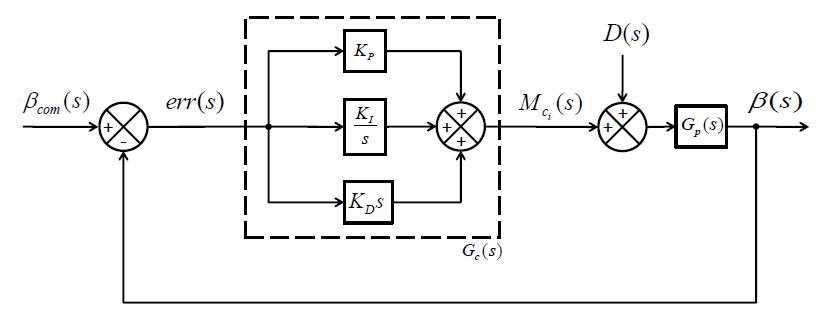
\includegraphics[scale=0.75]{img/pid_controller.PNG}
	\end{center}
	\fonte{Adaptado de \citeonline{Verma2018}.} 
\end{figure}


\begin{figure}[htb]
	\caption{Representação do Modelo de Controlador PID com distúrbios}
	\begin{center}
	    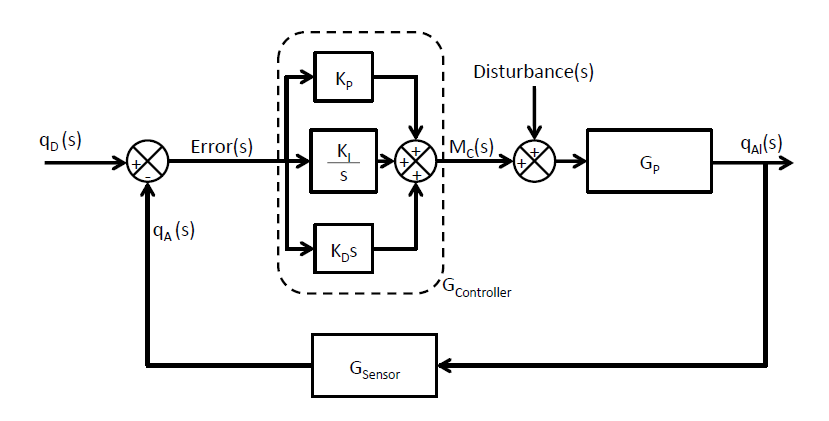
\includegraphics[scale=0.75]{img/pid_disturbe}
	\end{center}
	\fonte{Adaptado de \citeonline{Verma2018}.} 
\end{figure}


\subsection{INTELIGÊNCIA ARTIFICIAL}

\subsection{SISTEMA EMBARCADO}

\section{ESTADO DA ARTE}

\subsection{SISTEMAS INTELIGENTES DE SINTONIA AUTOMÁTICA} 
\chapter{Metodologia}

%%%%%%%%%%%%%%%%%%%%%%%%%%%%%%%%%%%
\section{Sistemas de Controle}

\subsection{Modelo Motor DC}
\begin{figure}[H]
  \caption{Modelo do Motor DC}
  \begin{center}
      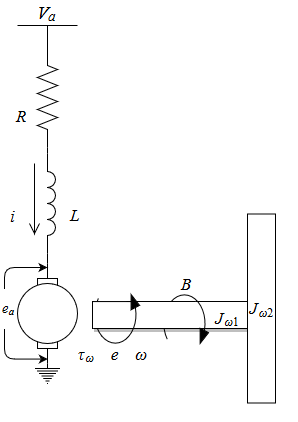
\includegraphics[scale=.8]{img/modelo_motor_dc}
  \end{center}
  \fonte{Elaborado pelo Autor.} 
  \label{fig:modelo_motor_dc}
\end{figure}

\subsection{Modelo Completo do Satélite}

\begin{figure}[H]
  \caption{Modelo em malha aberta}
  \begin{center}
      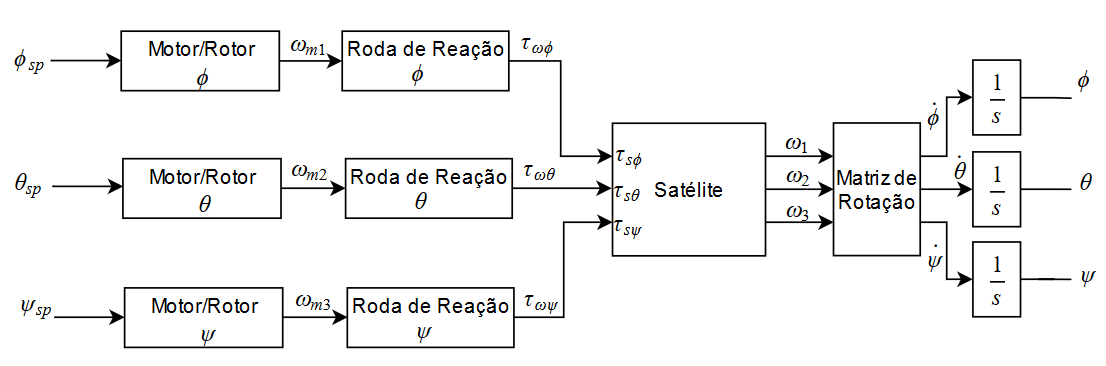
\includegraphics[scale=.55]{img/modelo_satelite_malha_aberta}
  \end{center}
  \fonte{Elaborado pelo Autor.} 
  \label{fig:modelo_satelite_malha_aberta}
\end{figure}


\begin{figure}[H]
  \caption{Modelo em malha fechada e com um Controlador PID}
  \begin{center}
      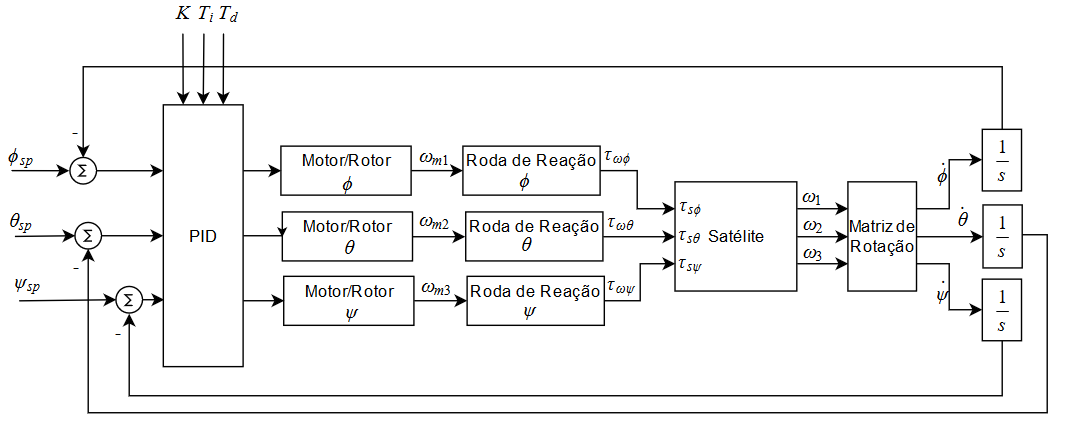
\includegraphics[scale=.55]{img/modelo_satelite_pid}
  \end{center}
  \fonte{Elaborado pelo Autor.} 
  \label{fig:modelo_satelite_pid}
\end{figure}


%%%%%%%%%%%%%%%%%%%%%%%%%%%%%%%%%%%%%%%%%%%%%%%%%%%%%%%%%%%%%%%%%%%%%%
\section{Software}

\begin{figure}[H]
  \caption{Topologia de Rede}
  \begin{center}
      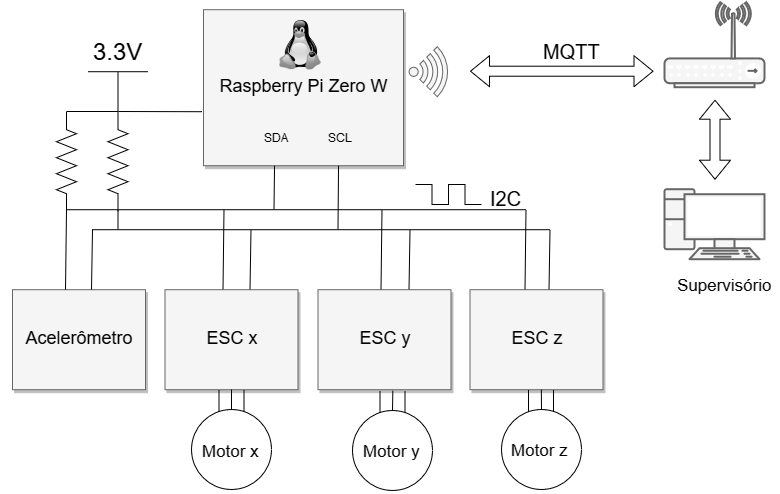
\includegraphics[scale=.75]{img/comunicacao_projeto}
  \end{center}
  \fonte{Elaborado pelo Autor.} 
  \label{fig:comunicacao_projeto}
\end{figure}

%%%%%%%%%%%%%%%%%%%%%%%%%%%%%%%%%%%
\subsection{Implementação do Controlador PID}

%%%%%%%%%%%%%%%%%%%%%%%%%%%%%%%%%%%
\subsection{Implementação da Rede Neural}

%%%%%%%%%%%%%%%%%%%%%%%%%%%%%%%%%%%
\subsection{Protocolos de Comunicação}

%%%%%%%%%%%%%%%%%%%%%%%%%%%%%%%%%%%
\subsection{Sistemas Supervisórios}


%%%%%%%%%%%%%%%%%%%%%%%%%%%%%%%%%%%%%%%%%%%%%%%%%%%%%%%%%%%%%%%%%%%%%%
\section{Hardware}


%%%%%%%%%%%%%%%%%%%%%%%%%%%%%%%%%%%
\subsection{Modelagem Motor DC e Rodas de Reação}

\begin{figure}[H]
  \caption{Desenho mecânico do conjunto Motor-Roda}
  \begin{center}
      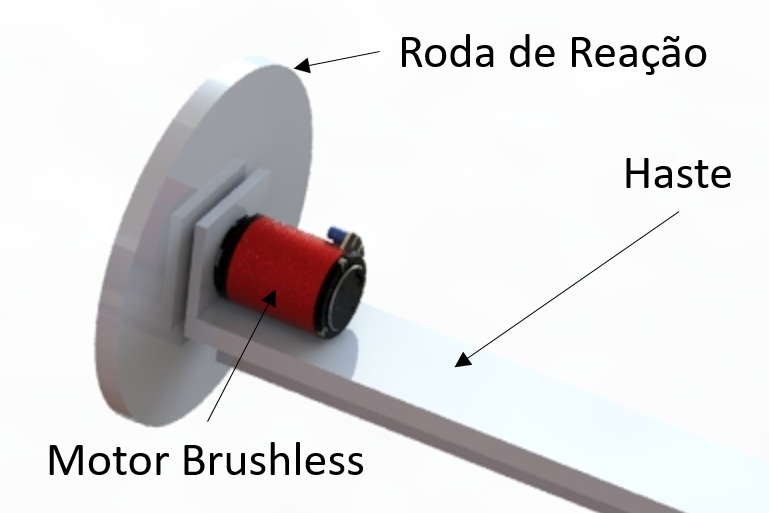
\includegraphics[scale=.45]{img/motor_roda_desenho}
  \end{center}
  \fonte{Elaborado pelo Autor.} 
  \label{fig:motor_roda_desenho}
\end{figure}


%%%%%%%%%%%%%%%%%%%%%%%%%%%%%%%%%%%
\subsection{Mancal a Ar}

\begin{figure}[H]
  \caption{Desenho Mecânico do Mancal a Ar}
  \begin{center}
      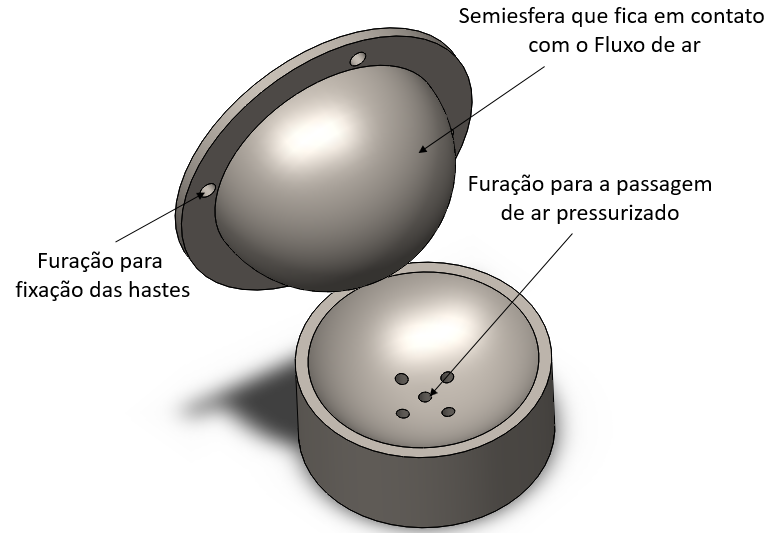
\includegraphics[scale=.45]{img/base_desenho}
  \end{center}
  \fonte{Elaborado pelo Autor.} 
  \label{fig:base_desenho}
\end{figure}


%%%%%%%%%%%%%%%%%%%%%%%%%%%%%%%%%%%
\subsection{Corpo do Simulador de Satélites}

\begin{figure}[H]
  \caption{Desenho Mecânico do Satélite Completo}
  \begin{center}
      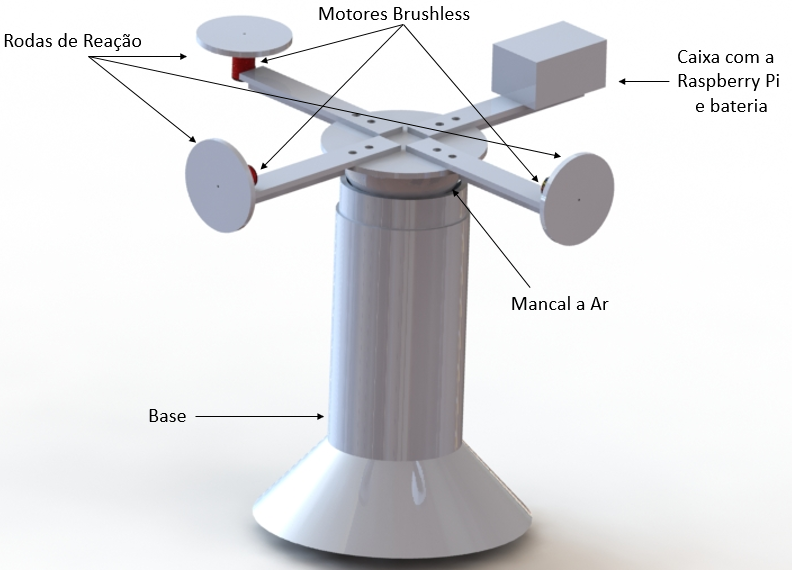
\includegraphics[scale=.75]{img/satelite_completo}
  \end{center}
  \fonte{Elaborado pelo Autor.} 
  \label{fig:satelite_completo}
\end{figure}

%%%%%%%%%%%%%%%%%%%%%%%%%%%%%%%%%%%
\subsection{Elementos Eletrônicos}

\begin{figure}[H]
  \caption{Raspberry Pi Zero}
  \begin{center}
      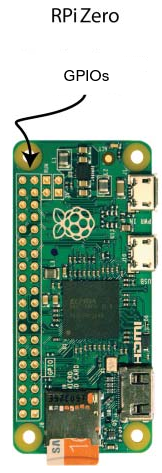
\includegraphics[scale=.55]{img/rasp_zero}
  \end{center}
  \fonte{Adaptado de \citeonline{Molloy2016}} 
  \label{fig:rasp_zero}
\end{figure}


\begin{figure}[H]
  \caption{Circuito impresso com o acelerômetro MMA7260QT}
  \begin{center}
      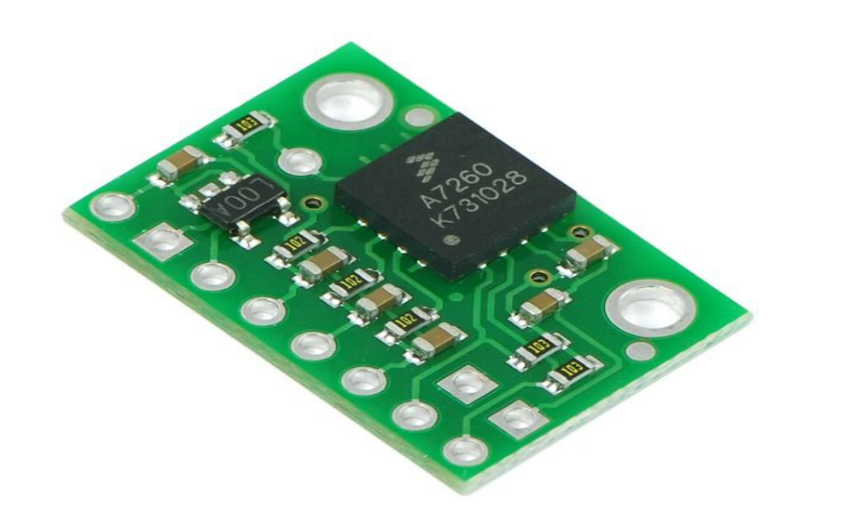
\includegraphics[scale=.45]{img/pci_acelerometro_calache_p22}
  \end{center}
  \fonte{Calache, Danilo Carreiro} 
  \label{fig:pci_acelerometro_calache_p22}
\end{figure}

\chapter{Cronograma}

\lipsum[23-27]
\phantompart
%% ||||||||||||||||||||||||||||||||||||||||||||||
% Capitulo de análise dos resultados
% ||||||||||||||||||||||||||||||||||||||||||||||
%\chapter{Análise dos Resultados}

%\lipsum[21-22]

% ----------------------------------------------
% Finaliza a parte no bookmark do PDF para que se inicie o bookmark na raiz e adiciona espaço de parte no Sumário
% ----------------------------------------------
% ----------------------------------------------
% CONCLUSÃO
% ----------------------------------------------
\chapter[Considerações Finais]{Considerações Finais}


% ==============================================
% ELEMENTOS PÓS-TEXTUAIS
% ==============================================
\postextual
% ==============================================
% Referências bibliográficas
% ==============================================
\bibliography{references}
% ==============================================
% Glossário
% ==============================================
\glossary
% ||||||||||||||||||||||||||||||||||||||||||||||
% Apêndices
% ||||||||||||||||||||||||||||||||||||||||||||||
\begin{apendicesenv}
\partapendices
% ----------------------------------------------
% Apêndice 1
% ----------------------------------------------
\chapter{Código em C}
  \begin{lstlisting}
    #include <stdio.h>

    void main(void)
    {
    	return 0;
    }
  \end{lstlisting}
\end{apendicesenv}
% ||||||||||||||||||||||||||||||||||||||||||||||
% ANEXOS
% ||||||||||||||||||||||||||||||||||||||||||||||
\begin{anexosenv}
\partanexos
% ----------------------------------------------
% Anexo 1
% ----------------------------------------------
\chapter{Datasheet}\label{anexo1}
%\includepdf[pages=-]{pdfs/Datasheet.pdf}%
\end{anexosenv}
% ==============================================
% INDICE REMISSIVO
% ==============================================
%\phantompart
%\printindex
% ----------------------------------------------
\end{document}